\chapter{Methodology}
\label{ch:methodology}
\glsresetall

\section{Targets}

  Five target models were chosen for this experiment. Each model is a missile-surrogate with a shared fuselage, and a unique nose cone. The dimensions of the fuselage and the nose cones are listed in table \ref{tab:models}. Nose cones 1-3 are simple cones with a fixed base diameter and edge length. Nose cones 4 and 5 are curved. They share the common 3 inch base diameter, with  differing diameters as they extend from the base to tip. The additional measurements represent the diameter of the cone at equally spaced intervals along the edge from base to tip. Each model is made of aluminum as is assumed to behave as a PEC in the presence of EMR. The Cad models of each missile nose is shown in figures \ref{nose_1_2}, \ref{nose_3_4}, and \ref{nose_5}. The side and top view of the missile is shown in figure \ref{fig:missile_body}.

  \begin{figure}[htbp]
    \centering
    \begin{subfigure}{.5\textwidth}
      \centering
      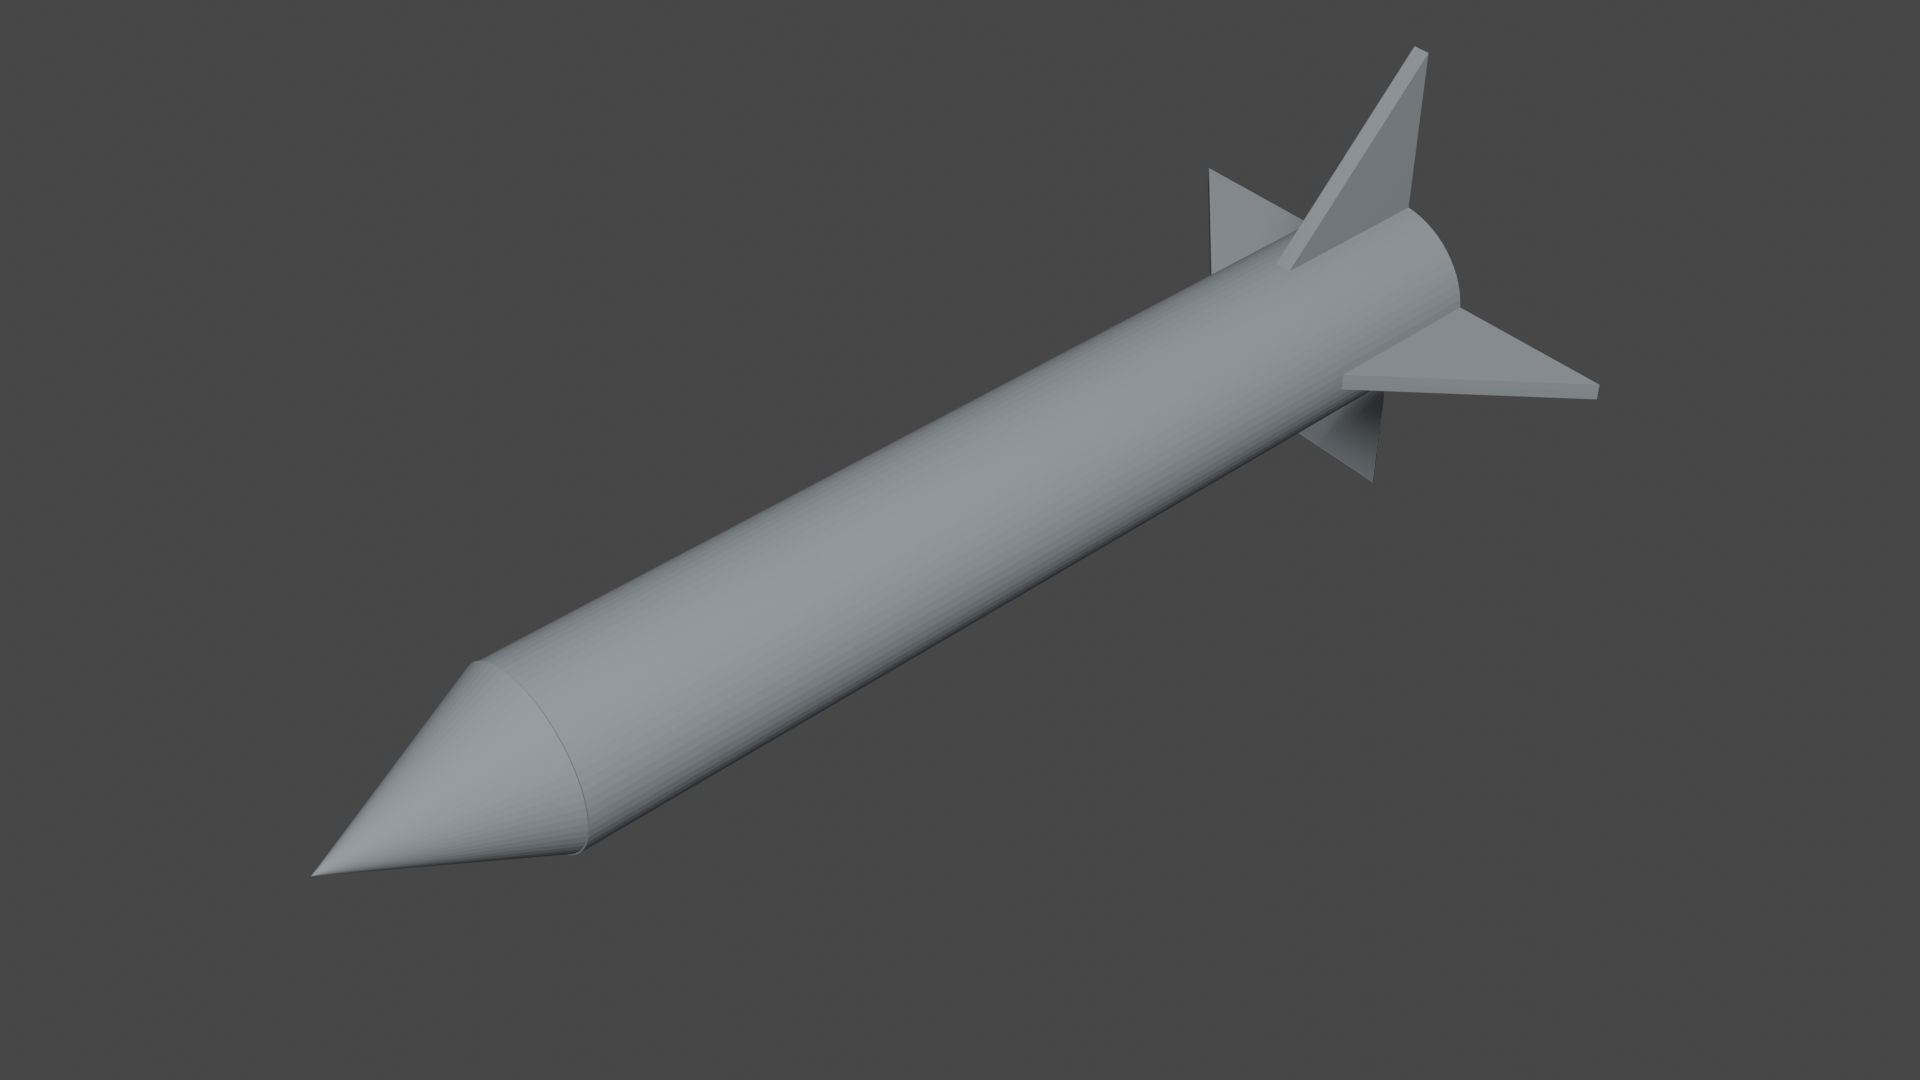
\includegraphics[width=.8\linewidth]{msl_side.png}
    \end{subfigure}%
    \begin{subfigure}{.5\textwidth}
      \centering
      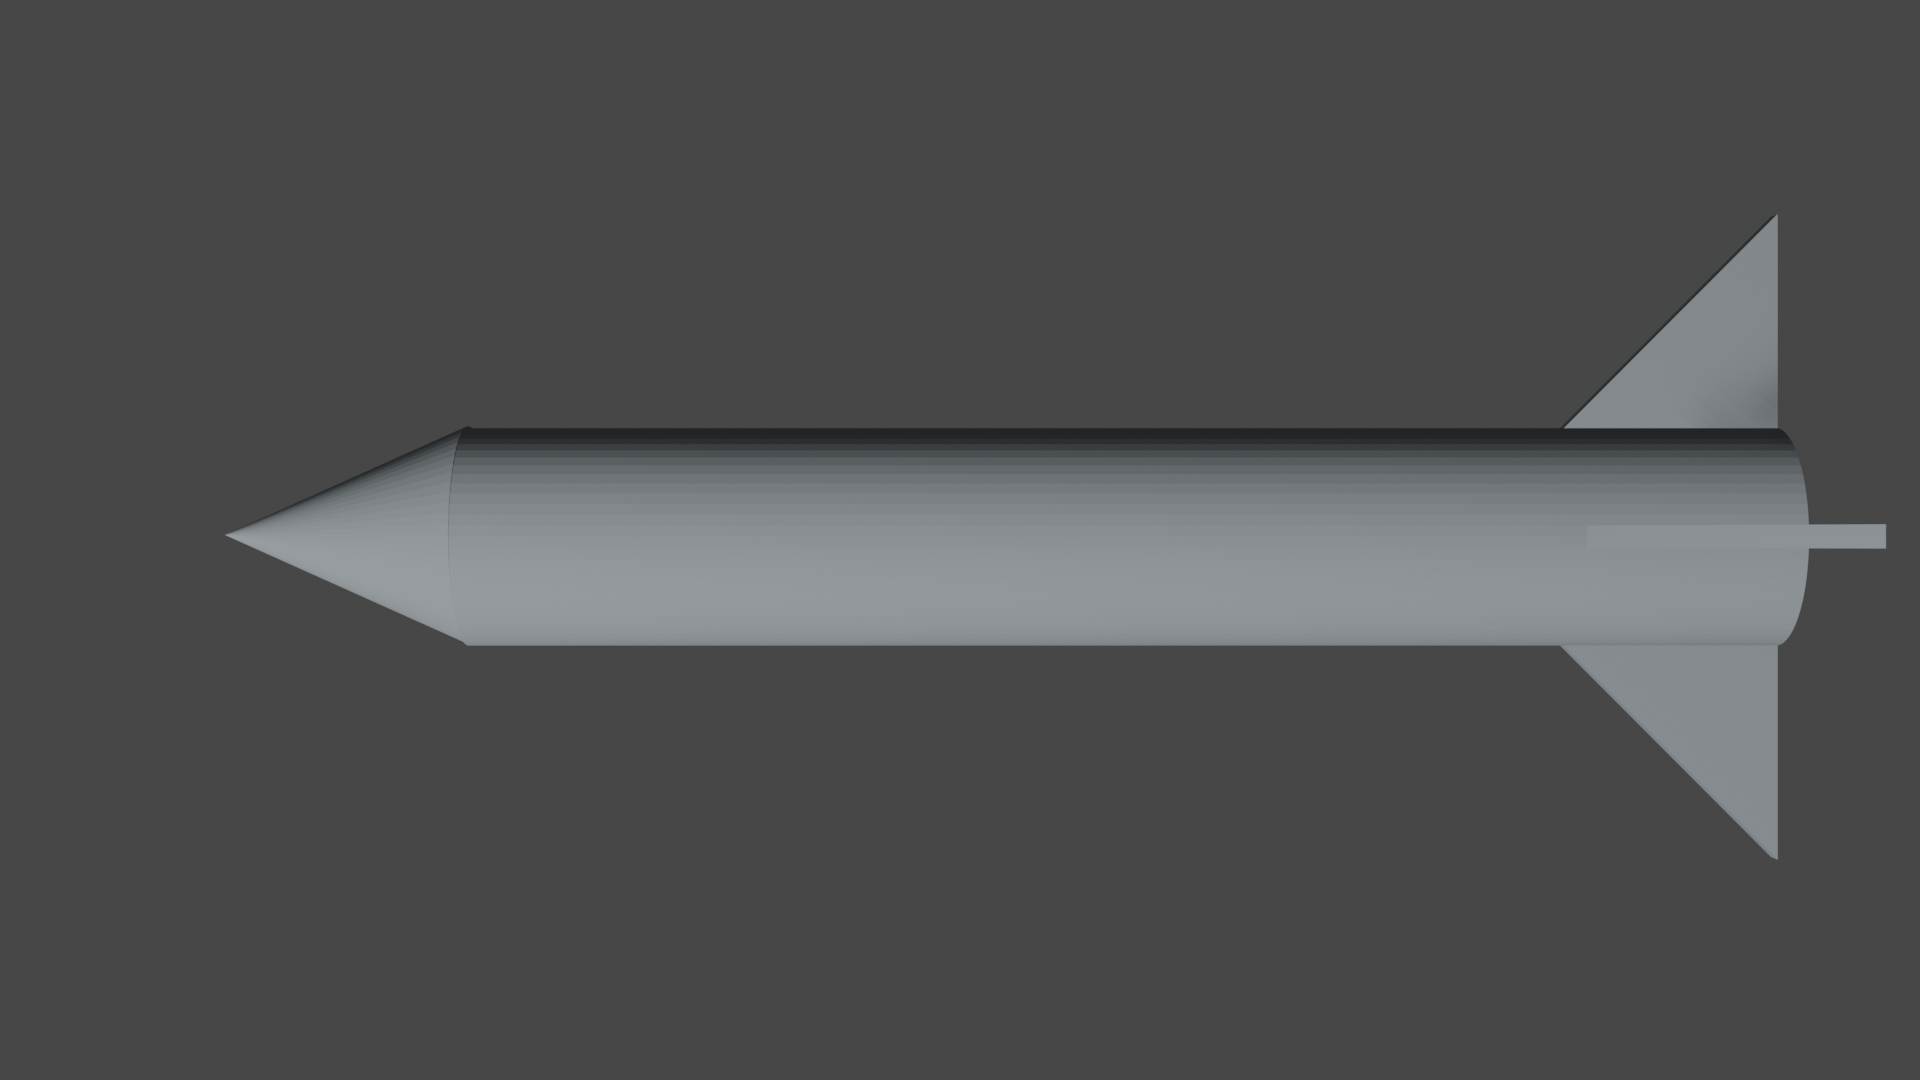
\includegraphics[width=.8\linewidth]{msl_top.png}
    \end{subfigure}
    \caption{Side and top view of the missile surrogate (Cad model)}
    \label{fig:missile_body}
  \end{figure}



  % TODO: Insert photos of the nose cones, and body assembly.

\section{Measurement}
  The targets were measured at the Air Force Institute of Technologies (AFIT) Compact Radar Range. The layout of the AFIT range is shown in figure \ref{fig:range}. The range uses a BlueMax G6 instrumentation radar (blue items in schematic), with a Vivaldi wide-band antenna configured in both horizontal and vertical polarizations. Transmitted signals are directed at a cruved reflector located 3 meters from the antenna. Ideally, the incident field will be a plane wave. That is, the wave front is the same when measured vertically or horizontally. However, the short distance between the antenna and the target will produce a curved wave-front surface. The reflector helps to `flatten' the wave front, and make it appear more planer.

  Targets are placed on a foam column located 7 meters from the reflector. The column is 2 meters tall, and can rotate 360 degrees. Foam is used, as its intrinsic properties are similar to air, and do not contribute significantly to scene clutter.

  \begin{figure}[htbp]
    \centering
    \begin{subfigure}{.5\textwidth}
      \centering
      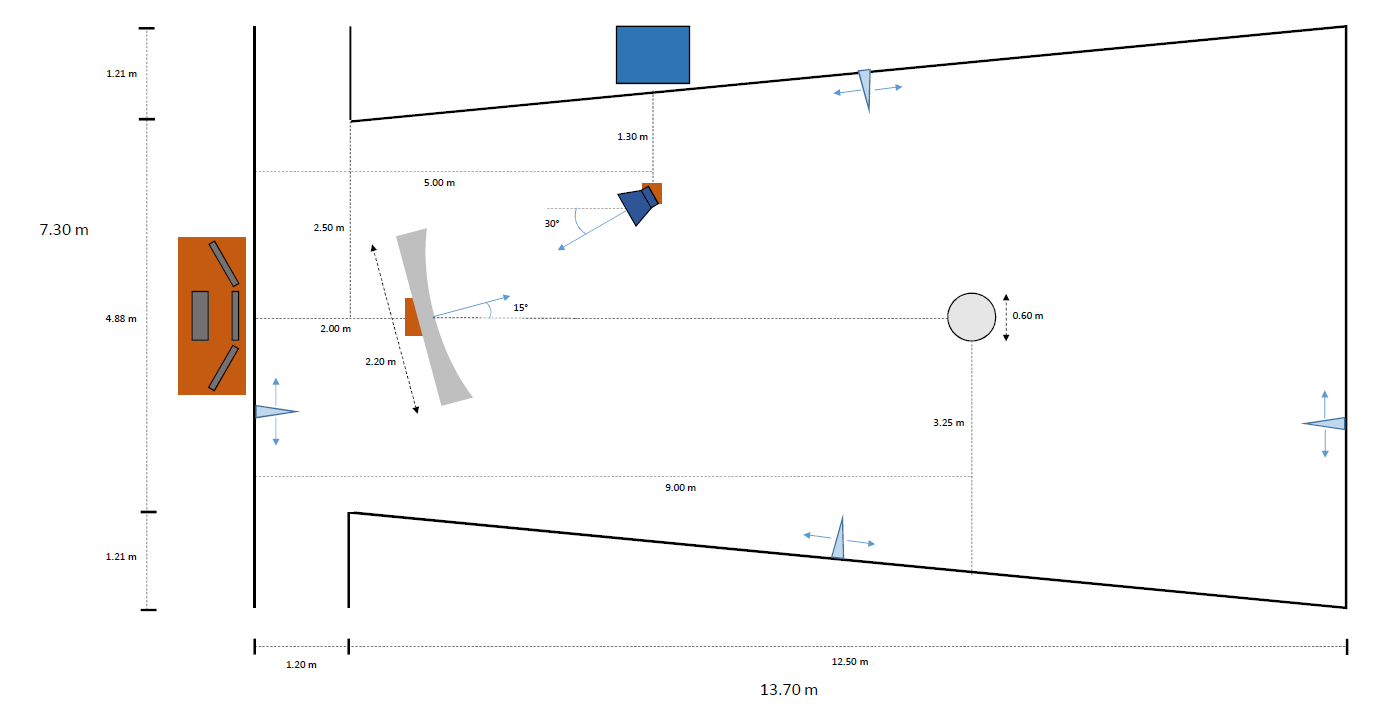
\includegraphics[width=.8\linewidth]{range.png}
    \end{subfigure}%
    \begin{subfigure}{.5\textwidth}
      \centering
      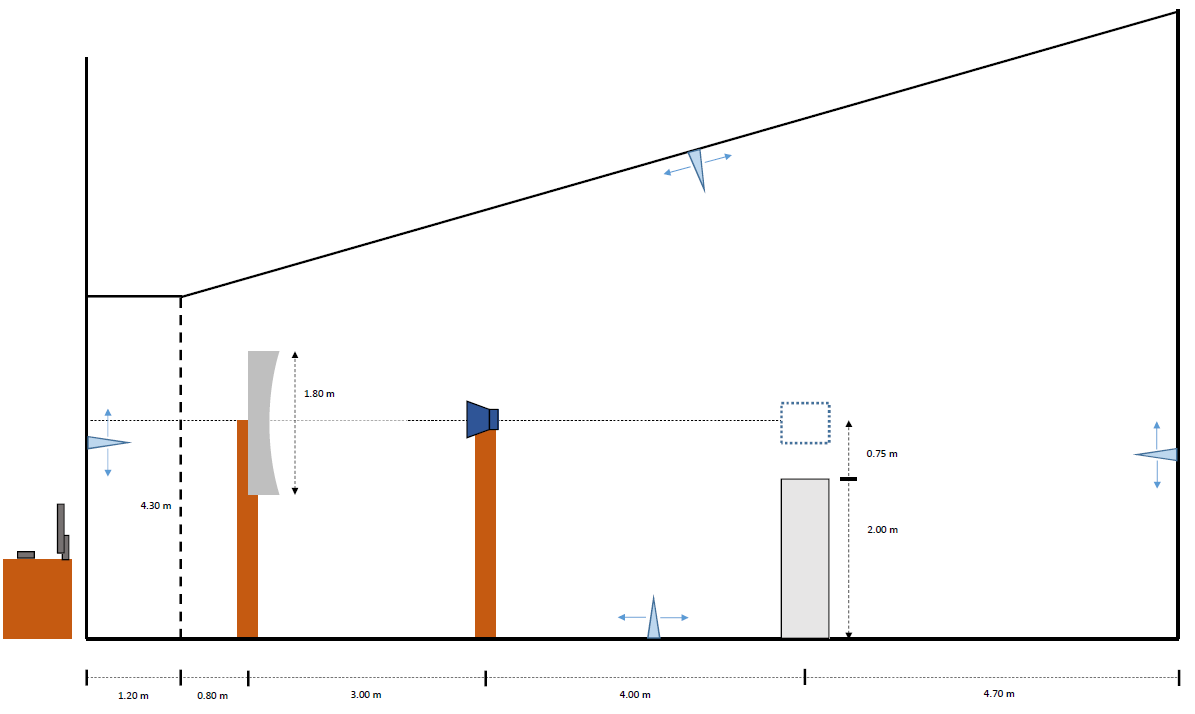
\includegraphics[width=.8\linewidth]{range_side.png}
    \end{subfigure}
    \caption[AFIT Compact Range Schematic]{Top-down and side view of the AFIT compact radar range.}
    \label{fig:range}
  \end{figure}

  The radar can capture measurements over multiple frequencies, polarizations, and target aspect-angles. Measurements are returned as complex voltages $M$. A measurement is collected using a specific carrier frequency $f$, at a single aspect angle $a$. For example, measurement $M_0$ is collected by launching a stream of pulses with carrier frequency $f_0$ at a target presenting a fixed aspect angle $a_0$. The receiver will collect and integrate $N$ echo pulses and store the value as $M(f_0, a_0)$. This process is repeated over the desired range of frequencies and angles resulting in a matrix

  \begin{equation}\label{eq:RCS_mat}
    E_{tt} =
     \begin{bmatrix}
       M_{0,0} & M_{0,1} & \cdots & M_{0,A} \\
       M_{1,0} & M_{1,1} & \cdots & M_{1,A} \\
       \vdots  & \vdots  & \ddots & \vdots  \\
       M_{F,0} & M_{F,1} & \cdots & M_{F,A}
     \end{bmatrix}
     \\
     E_{pp} =
      \begin{bmatrix}
      M_{0,0} & M_{0,1} & \cdots & M_{0,A} \\
      M_{1,0} & M_{1,1} & \cdots & M_{1,A} \\
      \vdots  & \vdots  & \ddots & \vdots  \\
      M_{F,0} & M_{F,1} & \cdots & M_{F,A}
      \end{bmatrix}
  \end{equation}

  where $E_{tt}$ and $E_{pp}$ represent measurements taken for the vertical and horizontally aligned incident wave polarization. Each row in the matrices corresponds to 360 aspect angles measured at one frequency. The total array shape is $F \times A$, where $F$ and $A$ are the number of frequencies and angles captured respectively.

  Table \ref{tab:m_params} lists the measurement parameters used for this experiment.

  \begin{table}
    \centering
    \begin{tabular}{lr}
      Transmitter Power: & $40$[dBm]\\
      Tx Gain: $15$[dB]\\
      Rx Gain: $15$[dB]\\
      IF BW: $200$[kHz]\\
      Noise Figure, $F$:  $3$[dB]\\
      Tx Loss: $4.5$[dB]\\
      Rx Loss: $4.5$[dB]\\
      Operating Temp: $68$[F]\\
      Pulse Width: & $10[ns]$\\
      Frequency Range: & $4.5-5.5 [GHz]$, $10 [MHz]$ step\\
      Aspect-angle Range: & $0-360 ^{\circ}$, $1^{\circ}$ step\\
      Integration Factor: & $1024$ \\
    \end{tabular}
    \caption{Measurement parameters.}
    \label{tab:m_params}
  \end{table}

  The radar used for this project produces a discrete RCS measurement at individual frequencies as opposed to a time domain response for each pulse. Since this time-domain information was unavailable, this experiment attempts to recreate the time-domain response, by capturing discrete measurements for each frequency and stitching them together into a frequency domain equivalent for the expected time-domain response.

  The integration factor was chosen to provide sufficiently accurate measurements. This ideal measurement serves as a signal to noise performance baseline.

  \subsection{Calibration}
    \label{sec:cal}
    Open air measurements must account for two distinct error sources:  range intrusion, and instrument calibration. Range intrusion accounts for spurious echo's from the floor, walls, target mount, and other physical objects in the range that interact with the incident field. These signals constitute the `background' of the scene and can be mitigated in two ways:  1. gating returns at the receiver to create quiet zones; 2. Implementing background subtraction using

    \begin{equation}
      E_{t, true} = E_{t, raw} - E_{t, bg}
    \end{equation}

    where $E_{t, raw}$ and $E_{t, bg}$ are measurements of the scene with and without the target in place. While background subtraction will help to reduce spurious signals, it cannot account for target-mount interactions and will not completely eliminate spurious returns.

    The instrument radar is calibrated using the substitution method:  a simple target whose RCS can be readily calculated is used to create a proportionality constant which accounts for deviations in radar performance \cite{Knott}. Since the range distances are fixed, the only factor of the radar range equation that will change is either the target's RCS, or fluctuation in transmitted power over frequency. By measuring a target with a known RCS, the proportionality constant $C$ can determined using

    \begin{equation}
      C = \frac{E_{cal, sim}}{E_{cal, raw} - E_{cal, bg}}
    \end{equation}

    where $E_{cal, raw}$ and $E_{cal, bg}$ are measurements of the scene with and without the calibration target respectively. The term $E_{cal, sim}$ is the RCS measurement of the calibration target. This experiment utilizes a 7 inch calibration cylinder whose RCS is modeled using CADFeko. Notably, the substitution method employs background subtraction as discussed previously.

    Prior to data processing, all target measurements are calibrated using

    \begin{equation}
      E_{t, true} = \frac{E_{t, raw} - E_{t, bg}}{E_{cal, raw} - E_{cal, bg}}
    \end{equation}

  \subsection{Measurement Results}

    Figures \ref{fig:n1}, \ref{fig:n2}, \ref{fig:n3}, \ref{fig:n4}, and \ref{fig:n5} represent the calibrated RCS measurements of missiles 1, 2, 3, 4, and 5 respectively. Each figure include a plot of the vertically and horizontally polarized radar configuration.

    The measured values are converted to RCS for the purpose of display using \ref{eq:ieee_rcs}, with a transmitted signal of $E_t = 1 [V/m^2]$, and converted to $RCS [dB_{sm}]$ using

    \begin{equation}
      RCS [dB] = 10 * \log \left( \frac{RCS [m^2]}{1 [m^2]}\right)
    \end{equation}

    The green sector represent the RCS data that is used to train the machine learning model. The RCS polar plots show only one frequency. The total frequency content of each target over all angles are shown in figures \ref{fig:c1}, \ref{fig:c2}, \ref{fig:c3}, \ref{fig:c4}, and \ref{fig:c5}. Again, figures are shown in $RCS [\textrm{dB}_{sm}]$ represent the calibrated RCS measurements of missiles 1, 2, 3, 4, and 5 respectively. Each figure include a plot of the vertically and horizontally polarized radar configuration.

\section{Simulation}

  Simulations were completed using Altair's CADFeko program. CADFeko uses an iterative Method of Moments - Surface Equivalent Principle (MoM, SEP) algorithm to compute the RCS response of the target model. Method of Moments is used to calculate scattering for targets in the Resonant regime:  target size is approximately on the same order as the incident wave length, but less than 10 times larger. [CITE SOMETHING FOR MOM, \cite{Knott}]. At 5 GHz, the incident wave length is 60 millimeters. At 457mm, the fuselage body is 7.62 times larger than the 5 GHz wavelength placing towards the upper end of the resonant regime. The smaller nose cones, ranging from 101 to 228 mm fit more comfortably into the resonant regime.

  Models were developed in Blender 3d. Models were exported from blender as .stl mesh objects, and imported into FreeCAD where they were converted to solids, and again exported as .step geometries. CADFeko must develop its own mesh for the imported geometries based on the requested frequency simulation range. Converting objects from a .stl mesh, to a .step geometry was the smoothest way to convert models into CADFeko friendly geometries given the authors limited experience with computer aided design.

  \subsection{Simulation Results}

    Figures \ref{fig:ns1}, \ref{fig:ns2}, \ref{fig:ns3}, \ref{fig:ns4}, and \ref{fig:ns5} represent the simulated RCS of missiles 1, 2, 3, 4, and 5 respectively. Each figure include a plot of the vertically and horizontally polarized radar configuration.


\section{Data Processing}

  \subsection{Data Set Generation}
    In order to mimic the expected response of a radar pulse, training and test data sets are built by slicing the RCS matrices shown in equation \ref{eq:RCS_mat} column wise. The resulting vectors

    \begin{equation}\label{eq:F_vec}
      F_{tt}(f, a_n) =
       \begin{bmatrix}
         M_{0, a_n} & M_{1,a_n} & \cdots & M_{F,a_n}
       \end{bmatrix},\,\,
       \\
     F_{pp}(f, a_n) =
      \begin{bmatrix}
        M_{0, a_n} & M_{1,a_n} & \cdots & M_{F,a_n}
      \end{bmatrix}
      \\
    \end{equation}

    contain the measurements $M(f, a_n)$ for all frequencies $f$, at a specified angle $a_n$ for the vertical and horizontal polarizations respectively. Each vector corresponds to the frequency content of an integrated pulse stream for each pose angle of the target. The training data set can be made arbitrarily large by multiplying frequency slices and applying random additive noise with power $N_{train}$ to create variance in each sample.

    Each sample in the training data set is assigned a label that corresponds to the `sector' that each sample falls in. Sectors are chosen such that RCS characteristics specific to the target fall in the same sector. This experiment utilizes either 3 or 4 90-degree sectors centered on the nose, tail, and sides of the target. The three label case collapses the sides of the fuselage into a single label.

    Test data sets are built similarly:  frequency vectors  are extracted from the measurement array, and additive noise with power level $N_{test}$ is applied.

  \subsection{Data Augmentation}
  \label{sec:DA}

    During training, neural networks optimize their decision weights by utilizing an `optimizer'. An optimizer is a method of testing whether the network is adjusting it weights in a way that maximizes its ability to categorize the input data correctly. This experiment utilizes a Stochastic Gradient Descent optimizer (SGD). This method favors adjustments in the networks weights that push towards a minimization of error in categorization. Since this is a method that utilizes slopes, differentiation is employed. In order to prevent unnecessarily large slopes, data is augmented. There are two forms of data augmentation that are typically employed: standardization, and normalization.

    Standardization takes the maximum value in the current training array, and scales the entire array. This creates a data range between 0 and 1. Standardization of data in this experiment is done using

    \begin{equation}\label{eq:F_stan}
      F_{tt}(f, a_n) =
       \begin{bmatrix}
         M_{0, a_n} & M_{1,a_n} & \cdots & M_{F,a_n}
       \end{bmatrix} / max(F_{tt}(f, a_n))
    \end{equation}

    where the function $max()$ pulls the max value in the vector.

    Normalization extracts the mean and standard deviation of the vector and returns a `Z-Score' for the each cell in the array using

    \begin{equation}\label{eq:F_z}
      F_{tt}(f, a_n) =
       \frac{\left(
       \begin{bmatrix}
         M_{0, a_n} & M_{1,a_n} & \cdots & M_{F,a_n}
       \end{bmatrix}
        - \mu \right)}{\sigma}
    \end{equation}

    where $\mu$ is the mean value of the vector, and $\sigma$ is the standard deviation.

  \subsection{Comparison}

\section{Neural Network Development}




\section{RCS Calculation}
